\section{AFD Palabras con terminación 'ere'}
	\subsection{Descripción del problema}
	Desarrollar un autómata finito determinista capaz de encontrar las palabras con terminación 'ere' ya sea leyendo un archivo txt o en una linea de texto que el usuario ingresa, y que dichas palabras se muestren en pantalla y en el caso del archivo de texto imprimir la linea y el numero de palabra (por linea) en el que fue encontrada dicha palabra.
	Es importante señalar que todo aquello que no es un símbolo del alfabeto ingles, $ \sum =\lbrace a, b, ..., z, A, B, ..., Z \rbrace $, es tomado como un espacio. Además, debe tener una opción para visualizar el siguiente diagrama.
	\begin{figure}[H]
		\begin{center}
		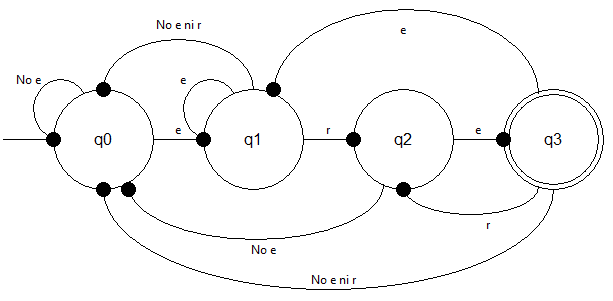
\includegraphics[width=14cm, height=7cm]{img/ere.png}
		\caption{Diagrama de transiciones del autómata 'ere'.}
		\label{fig:diagrama1}
		\end{center}
	\end{figure}
	\subsection{Código}
	El código fue realizado en Python 3.5.
	\subsection{Pruebas}
	Pruebas de las opciones del menú.
	\\
	{\large Modo de consola.}
	\begin{figure}[H]
		\begin{center}
			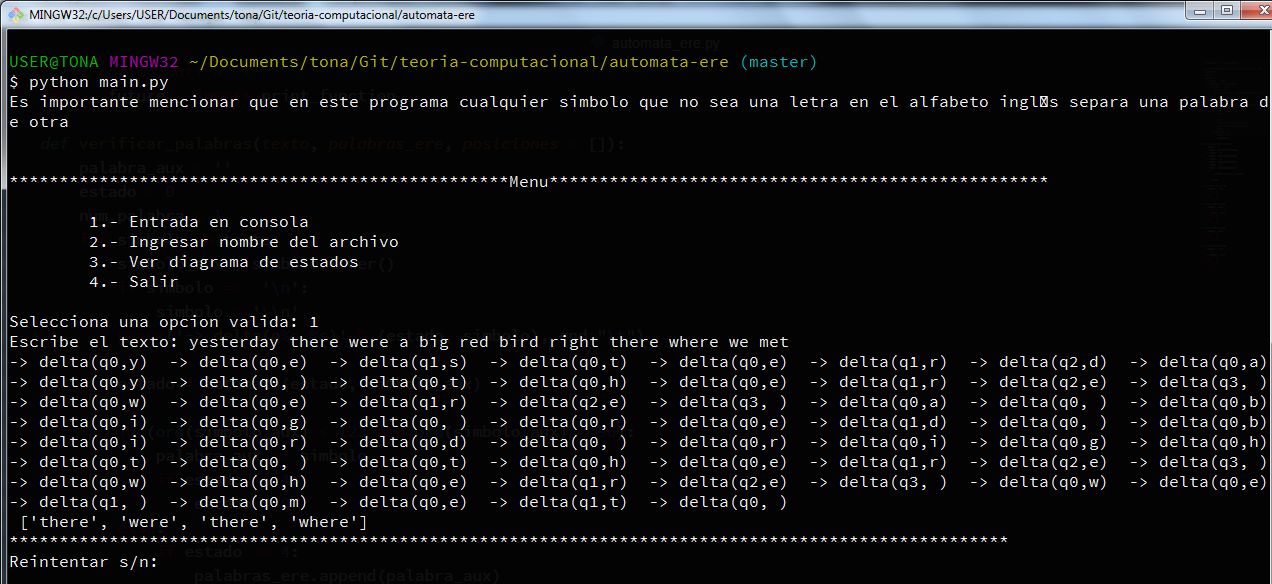
\includegraphics[width=\linewidth, height=7cm]{img/ere-manual.png}
			\caption{Historia del autómata y las palabras con terminación 'ere'.}
			\label{fig:ere1}
		\end{center}
	\end{figure}
	{\large Modo archivo.}
	\begin{figure}[H]
		\begin{center}
			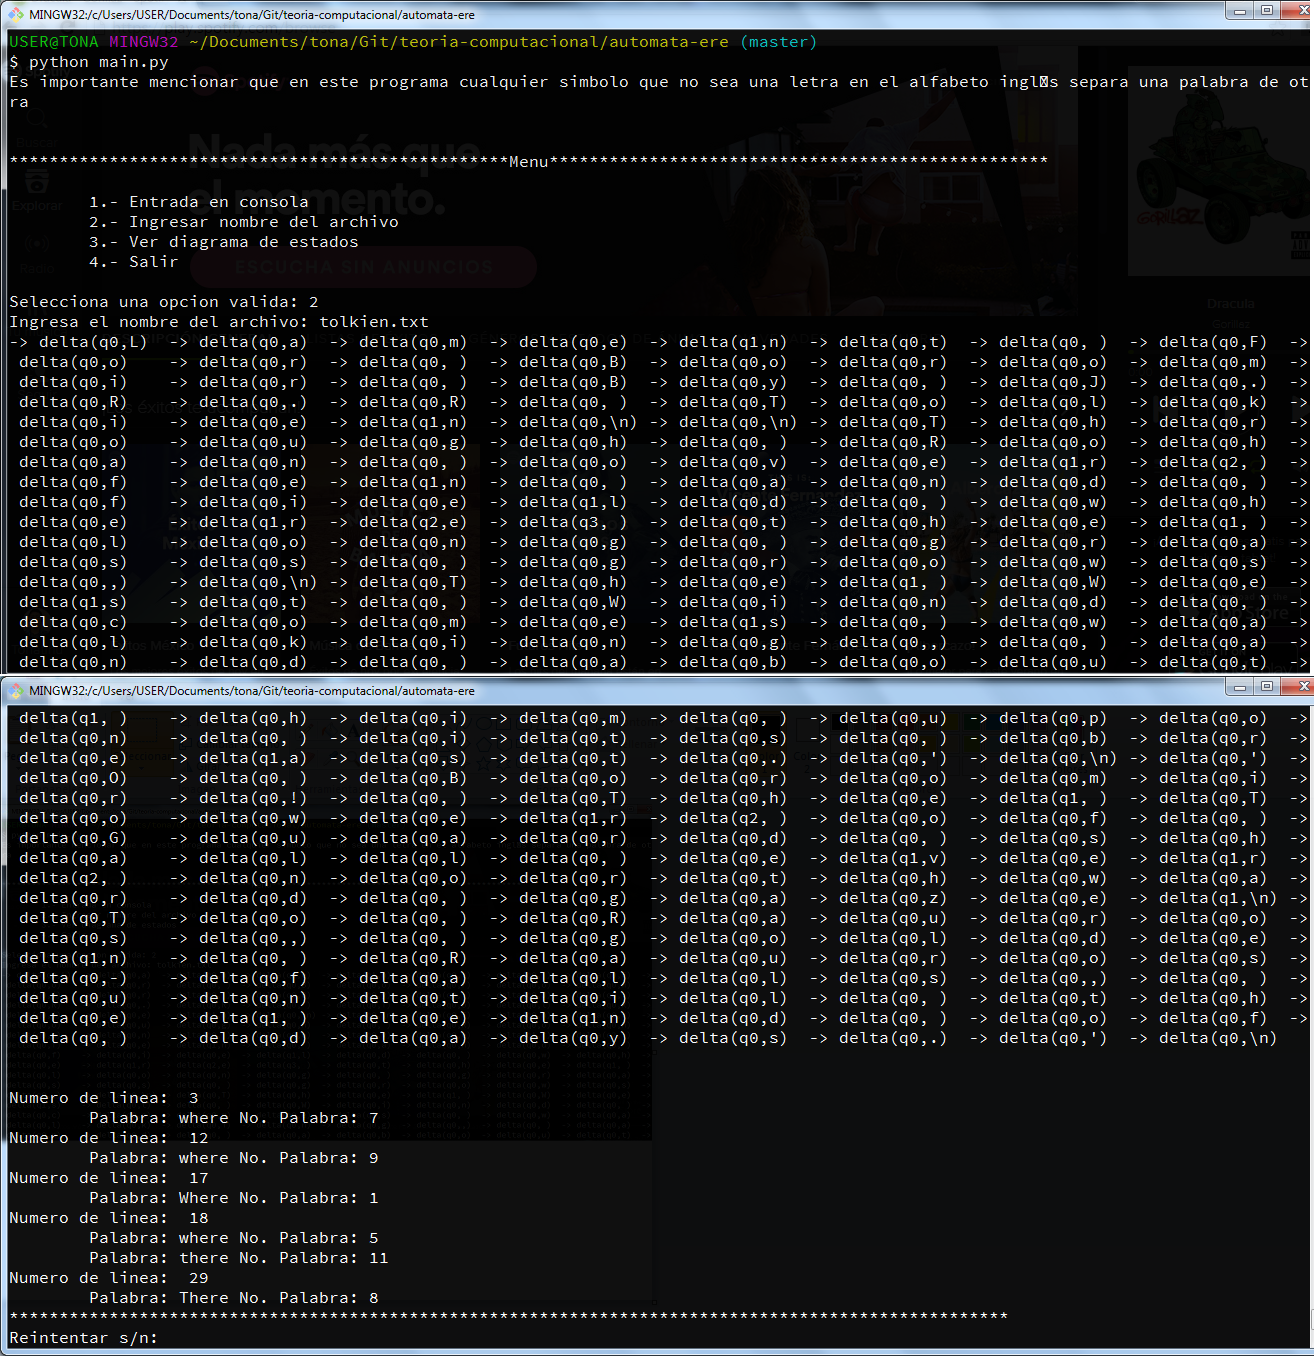
\includegraphics[width=\linewidth, height=17cm]{img/ere-automatico.png}
			\caption{Parte de la historia del autómata y las palabras con terminación 'ere'.}
			\label{fig:ere2}
		\end{center}
	\end{figure}
	{\large Diagrama.}
	\begin{figure}[H]
		\begin{center}
			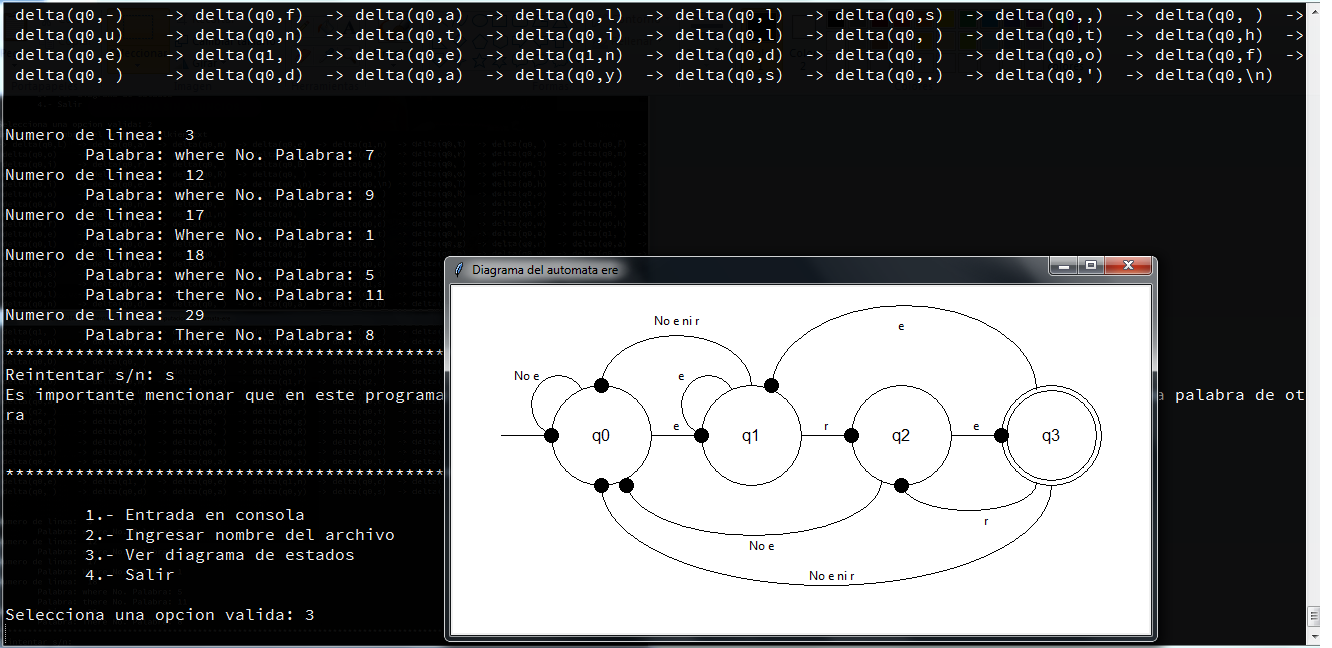
\includegraphics[width=\linewidth, height=7cm]{img/diagrama-ere.png}
			\caption{Diagrama de transiciones del autómata 'ere'.}
			\label{fig:ere3}
		\end{center}
	\end{figure}